\chapter{Projekt Systemy Homelab}

\section{Wymagania funkcjonalne i niefunkcjonalne}

\subsection{Wymagania funkcjonalne}

\begin{enumerate}
    \item \textbf{Zarządzanie infrastrukturą} - mozliwość konfiguracji i zarządzania maszynami wierualnymi oraz kontenerami Docker.
    \item \textbf{Panel administracyjny} - intuicyjny interfejs uzytkownika stworzony przy pomocy systemu AppSmith, do zarządzania zasobami systemu.
    \item \textbf{Baza danych} - przechowywanie informacji o konfiguracji systemu i uzytkownikach w MongoDB.
    \item \textbf{Bezpieczny dostęp zdalny} - integracja z Tailscale umozliwaiajca dostęp z dowolonego miejsca na ziemii.
    \item \textbf{Automatyzacja wdrozeń} - wsparcia dla CI/CD za pomocą GitHub Pipelines.
    \item \textbf{Obsługa domeny} - integracja z DuckDNS w celu dynamicznego zarządzania domeną.
    \item \textbf{Monitorowanie zasobów} - mechanizmy zbierania infromacji o wykorzystaniu CPU, pamięci RAM oraz przestrzeni dyskowej.
    \item \textbf{Wsparcie dla rozszerzeń} - mozliwość dodawania nowych funkcji poprzez kontenery Dockera.
    \item \textbf{Łatwe wdrazanie aplikacji} - opcja uruchamiania własnych usług w kontenerach bez konieczności zaawansowanej konfiguracji.
    \item \textbf{Bezpieczne uwierzytelnianie i automatyzacja} - mechanizm logowania oparty na OAuth2 i zarządzanie rolami uzytkowników.
\end{enumerate}

\pagebreak

\subsection{Wymagania niefunkcjonalne}

\begin{enumerate}
    \item \textbf{Niski pobór energii} - system wdrazany na Raspberry Pi 5, co zapeni efektywność energetyczną.
    \item \textbf{Wysoka dostępność} - redundancja i odporność na awarię dzięki Docker oraz Integracji z VPN.
    \item \textbf{Łatwość w utrzymaniu} - system powinien umozliwiac łatwe aktualizację i rekonfigurację w razie potrzeby ręcznej interwencji.
    \item \textbf{Skalowalność} - mozliwość rozszerzenia o nowe komponenty i usługi.
    \item \textbf{Bezpieczeństwo} - szyfrowanie komunikacji oraz kontrola dostępu do zasobów.
    \item \textbf{Modularność} - podział systemu na niezalezne komponenty działające w kontenerach Docker.
    \item \textbf{Integracja z open-source} - Wspracie dla narzędzi i trchnologii dostępnych na licencji open-source.
    \item \textbf{Minimalizacja kosztów} - niskie koszty sprzętowe i utrzymanie dzieki Raspberry Pi i rozwiązaniom chmurowym typu DuckDNS.
    \item \textbf{Wydajność} - optymalizacja aplikacji pod Raspberry Pi, aby zapenić płynne działąnie 
    \item \textbf{Łatwość wdrozenia} - uproszczona konfiguracja pozwalająca na szybkie uruchomienie systemu.
\end{enumerate}

\pagebreak

\section{Architektura systemu}
System HomeLab składa się z kilku kluczowych komponentów:

\subsection{Backend (FastAPI + MongoDB)}
\begin{itemize}
    \item FastAPI \cite{FastAPI} odpowiada za obsługę logiki biznesowej i API Backendu.
    \item MongoDB \cite{MongoDB} przechowuje dane uzytkowników, konfigurację systemowe i rejestr operacji.
\end{itemize}

\subsection{Frontend (AppSmith)}
\begin{itemize}
    \item niskokodowa platforma pozwalająca na łatwe budowanie interfejsu uzytkownika.
    \item Integracja z backendem poprzez REST API
\end{itemize}

\subsection{Warstwa sieciowa}
\begin{itemize}
    \item Połączenia umozliwione i zabezpieczone poprzez Tailscale (VPN).
    \item DuckDNS zapewniający mozliwość dostępu do systemu za pomocą domeny, zamiast adresu IP.
\end{itemize}

\subsection{Środowisko kontenerowe}
\begin{itemize}
    \item Docker wykorzystywany do zarządzania usługami systemu.
    \item Mozliwość łatwego wdrazania i skalowania aplikacji poprzez kontenery.
\end{itemize}

\subsection{Automatyzacja CI/CD}
\begin{itemize}
    \item GitHub Actions zarządza automatyzacją wdrozeń i aktualizacji systemu
    \item Kazda zmiana w kodzie uruchamia testy oraz wdrozenie nowych wersji aplikacji.
\end{itemize}

\subsection{Urządzenie docelowe}

Raspberry Pi 5 jako główny host systemu, zapewniający niskie zuzycie energii i optymalizację kosztów.

\begin{figure}
    \begin{center}
        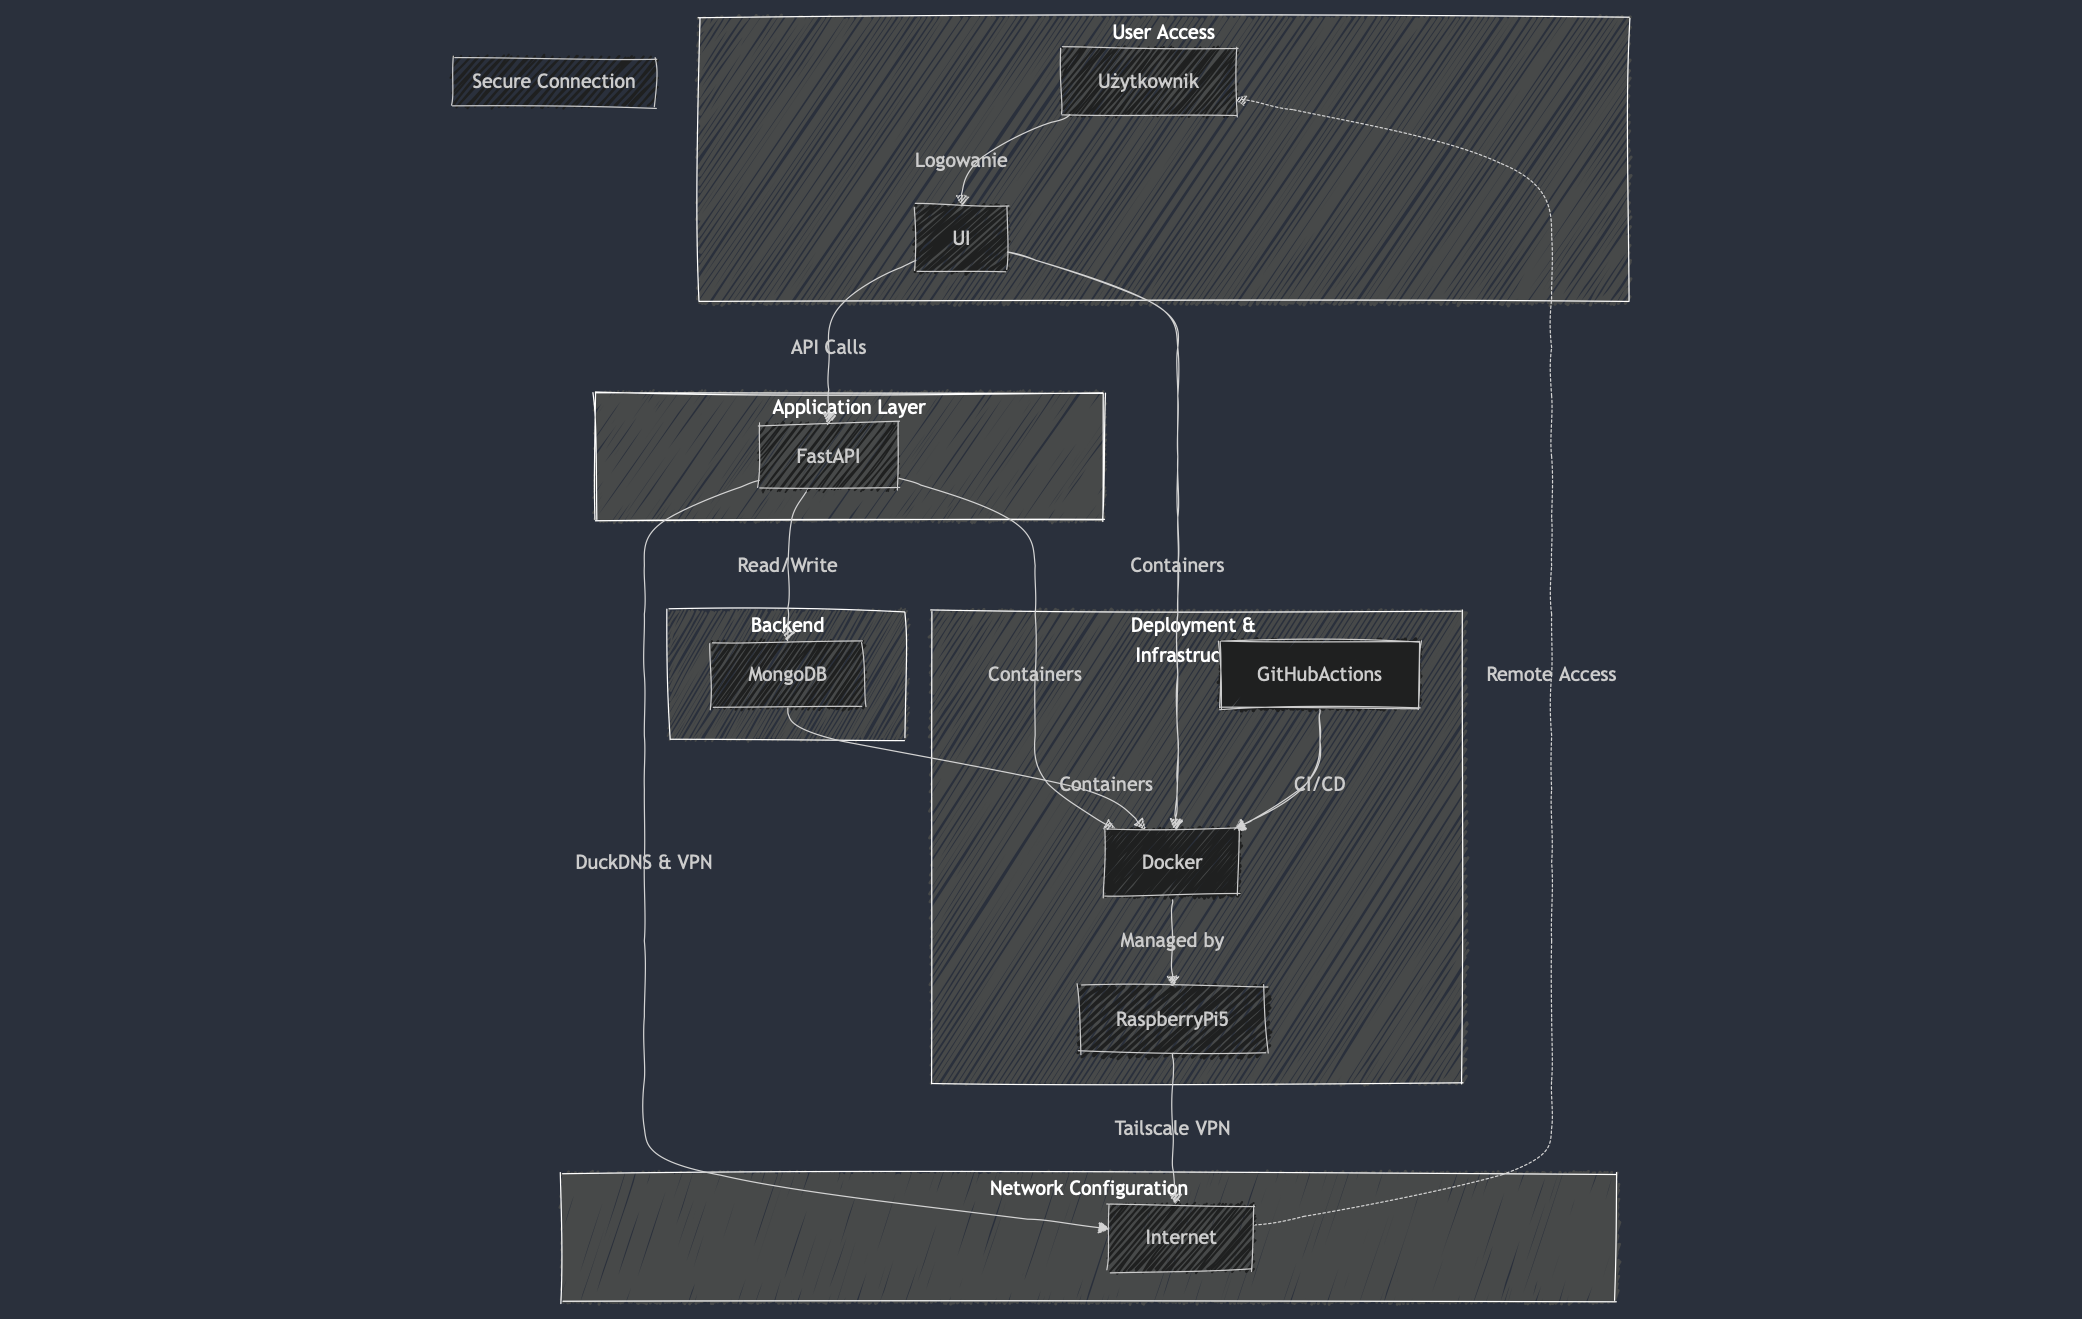
\includegraphics[width=0.9\textwidth]{./chapters/mermeid/schemat_architektury.png}
        \caption{Schemat Architektury}
    \end{center}
\end{figure}


\section{Technologie i narzędzia uzyte w systemie}

System HomeLab wykorzystuje następujące technologie:
\subsection{Backend}
\begin{itemize}
    \item FastAPI - szybki i nowoczesny framework do tworzenia API w pythonie
    \item MongoDB - baza danych NoSQL przechowująca konfigurację i dane uzytkowników
\end{itemize}
\subsection{Frontend}
\begin{itemize}
    \item AppSmith - niskokodowe narzędzia do budowy interfejsu uzytkownika.
    \item RestAPI - wykorzystywane do komunikacji między frontendem a backendem.
\end{itemize}
\subsection{Warstwa Sieciowa}
\begin{itemize}
    \item Tailscale - VPN do bezpiecznego zapewnienia zdalnego dostępu do systemu, bez konieczności posiadania stałego adresu IP.
    \item DuckDNS - dynamiczny system zarządzania domeną umozliwiający łatwy dostęp do systemi.
\end{itemize}
\subsection{Środowisko uruchomieniowe}
\begin{itemize}
    \item Docker - uzywany do konteneryzacji aplikacji i zarządzania zaleznościami.
    \item Raspberry Pi 5 - host systemu zapewniający energooszczędność i niski koszt.
\end{itemize}
\subsection{Automatyzacja CI/CD}
\begin{itemize}
    \item GitHub Actions - narzędzie do automatyzacji wdrozeń i testowania kodu.
    \item Pipeline CI/CD - automatyczne testowanie, budowanie i wdrazanie aplikacji
\end{itemize}

Dzięki zastosowaniu powyzszych technologii system Homelab będzie nowoczesnym, skalowalnym i energooszczędnym rozwiązaniem dla uzytkowników domowych.